\capitulo{5}{Resultados}

Se presentan a continuación las simulaciones llevadas a cabo en este estudio.

\section{Comportamiento glucémico óptimo}
\subsection{Insulina constante y variable}

En esta sección se presentan las gráficas resultantes de la simulación de los niveles de glucosa para un paciente sano (Tabla \ref{tab:valores_no_diabetico}) usando el Modelo de Bergman con insulina constante y variable en el organismo. La suposición inicial de insulina constante es meramente hipotética (pues los niveles de glucosa no son ctes.), pero representa de forma adecuada el modelado de la glucosa para esta condición. La respuesta a la simulación tras ingesta parte de una glucosa de 135 mg/dL.
Los escenarios considerados en la Figura \ref{fig:bergman_insulinas_comp} muestran el comportamiento de la glucosa, insulina e insulina activa tras una ingesta bajo dos casos: el primero de ellos, empleando una insulina constante, donde se espera que tanto I(t) como X(t) se mantengan estables en su mismo valor (la insulina activa en 0, pues no hay variación de I(t)). Para el segundo caso, al realizar estos escenarios aplicando una insulina variable, modelada en la Ecuación (\ref{eq:insulina_variable}), se muestra un comportamiento más próximo a la realidad del sistema biológico, donde los niveles presentan algo de oscilación. Además, se observará cómo varía la insulina a lo largo del tiempo, que alcanzará un pico cuando haya mucha glucosa en el organismo, y posteriormente se estabilizará en su nivel basal. La insulina activa, por su parte, también experimentará un aumento, consecuencia del aumento de la insulina. Una vez que finalice la variación de I(t), X(t) se estabilizará de nuevo.
\clearpage

\begin{figure}[htbp]
    \centering
    \begin{subfigure}[b]{0.9\linewidth} % Ancho ajustado al 90% del ancho de la línea
        \centering
        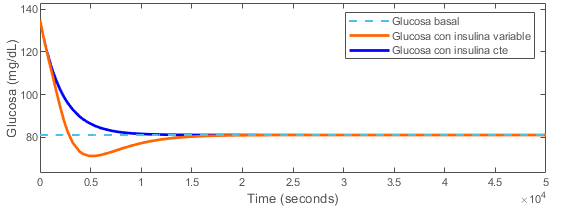
\includegraphics[width=\linewidth]{img/modelo_original/glucosa ins variable y no.png}
        \caption{Glucosa con insulina constante y variable.}
        \label{fig:bergman_glucosa}
    \end{subfigure}
    
    \vspace{0.5cm} % Espacio vertical entre las subfiguras

    \begin{subfigure}[b]{0.9\linewidth} % Ancho ajustado al 90% del ancho de la línea
        \centering
        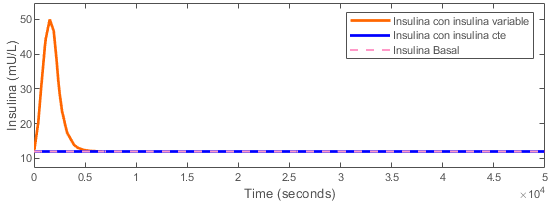
\includegraphics[width=\linewidth]{img/modelo_original/insulina ins variable y no.png}
        \caption{Insulina con insulina constante y variable.}
        \label{fig:bergman_insulina}
    \end{subfigure}

    \vspace{0.5cm} % Espacio vertical entre las subfiguras

    \begin{subfigure}[b]{0.9\linewidth} % Ancho ajustado al 90% del ancho de la línea
        \centering
        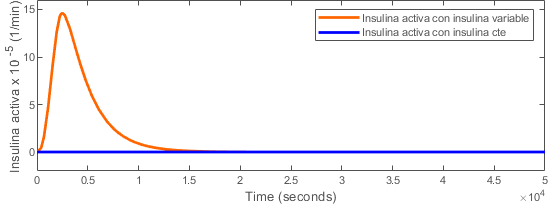
\includegraphics[width=\linewidth]{img/modelo_original/X_insvariable.png}
        \caption{Insulina activa con insulina constante y variable.}
        \label{fig:bergman_X}
    \end{subfigure}
    
    \caption{Comparativa del comportamiento de la glucosa, insulina e insulina activa tras una ingesta para una insulina constante y variable. Fuente propia.}
    \label{fig:bergman_insulinas_comp}
\end{figure}

\subsection{Variación de los parámetros del Modelo de Bergman}

Mientras que para la anterior simulación se ha seleccionado un umbral de liberación de insulina $p_5$ por parte del páncreas (Sección \ref{sec:p5})  de 90 mg/dL, se ha estudiado la \textbf{variación de este parámetro $p_5$} y su efecto en la respuesta de la glucosa. Se simulan cuatro casos, además del caso anterior ya realizado, con valores para $p_5$ de 81 mg/dL (igual que Gb), 85 mg/dL, 95 mg/dL y 100 mg/dL.
El resultado ha sido el siguiente:

\begin{figure}[htbp]
    \centering
    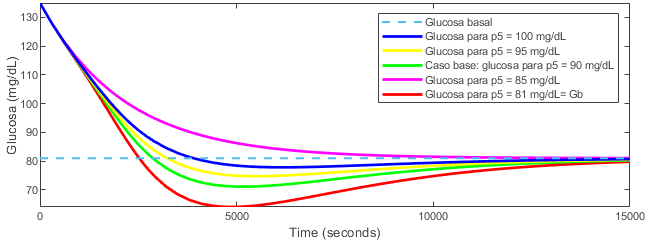
\includegraphics[width=0.9\linewidth]{img/modelo_original/p5_gluc.PNG}
    \caption{Efecto en la glucosa de la variación del umbral $p_5$. Fuente propia.}
    \label{fig:p5_gluc}
\end{figure}
\begin{figure}[htbp]
    \centering
    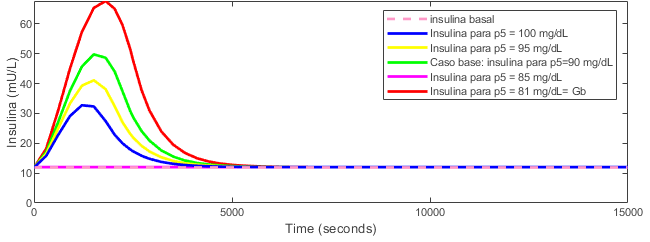
\includegraphics[width=0.9\linewidth]{img/modelo_original/p5_ins.PNG}
    \caption{Efecto en la insulina de la variación del umbral $p_5$. Fuente propia.}
    \label{fig:p5_ins}
\end{figure}

Para la glucosa, las diferencias no son muy significativas. Se observa que, de forma generalizada, que valores bajos de $p_5$ causan una menor pendiente en la estabilización de la curva de la glucosa. Aun así, la variación es escasa (pues rondan todos los supuestos valores comprendidos entre 70 y 75 mg/dL).
Para la insulina, se observa que valores más altos de $p_5$ hacen que la liberación de insulina finalice antes, pues el umbral es más alto, por lo que cuando G(t) <100, ya no se considera necesario liberar insulina. Esto hace por tanto que los niveles de insulina caigan antes a su nivel Ib. Valores más bajos de $p_5$ hacen que Ib se alcance levemente más tarde, debido a que la condición G(t) > $p_5$ sigue vigente más tiempo. El resultado es una curva cuyo tiempo de asentamiento es mayor a medida que p5 disminuye.
Valores muy bajos de p5, en este caso coincidentes con Gb (curva azul), suponen la aparición de unos niveles de insulina por debajo del basal. Tras la ingesta, y por el comportamiento variable de la insulina en el organismo, antes de estabilizarse la glucosa en su valor basal, sufre una leve disminución (ver Figura \ref{fig:p5_gluc}) inferior a Gb. Para un $p_5$ = Gb, cuando G(t)< Gb, el páncreas estima que no es necesario liberar insulina, por lo que los valores de esta caen abruptamente hasta rozar el 0.

Analizando el comportamiento del término (\ref{eq:termino_p5}) de la ecuación de la insulina (\ref{eq:insulina_variable}),

\begin{equation}
    termino = p_6 (G(t)-p_5)^+ t 
    \label{eq:termino_p5}
\end{equation}

se puede observar de manera más precisa el efecto de la variación del umbral $p_5$ en el organismo. Según lo indicado en esta ecuación (\ref{eq:termino_p5}), solo cuando la concentración de glucosa G(t) exceda el umbral $p_5$, el término completo será positivo y afectará a la insulina I(t). SI G(t) fuera menor que $p_5$, el término sería 0. Además, si G(t) > $p_5$, el término se multiplica por el tiempo, lo que sugiere un aumento de producción de insulina por el páncreas proporcional a la diferencia entre G(t) y $p_5$. Gráficamente se obtiene el mismo razonamiento en la Figura \ref{fig:termino_p5}.

\begin{figure}[htbp]
    \centering
    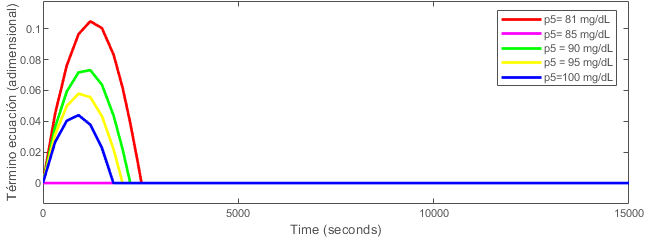
\includegraphics[width=0.9\linewidth]{img/modelo_original/p5_var/p5_termino.png}
    \caption{Comportamiento del término de la ecuación de la insulina para diferentes valores de p5. Fuente propia.}
    \label{fig:termino_p5}
\end{figure}

Acercando estas gráficas, y con la finalidad de mostrar la correlación entre este término y la glucosa respecto del tiempo, se ha calculado para la Figura \ref{fig:p5_gluc} en qué instante la glucosa G(t) para $p_5$ = 95 mg/dL alcanza dicho valor(G(t) = $p_5$ = 95 mg/dL). Se ha obtenido un tiempo t = 2030 s. Se muestra a continuación la Figura \ref{fig:zoom_p5} con el cursor establecido en este tiempo.  
\clearpage

\begin{figure}[htbp]
    \centering
    \begin{subfigure}[b]{0.9\linewidth} % Ancho ajustado al 90% del ancho de la línea
        \centering
        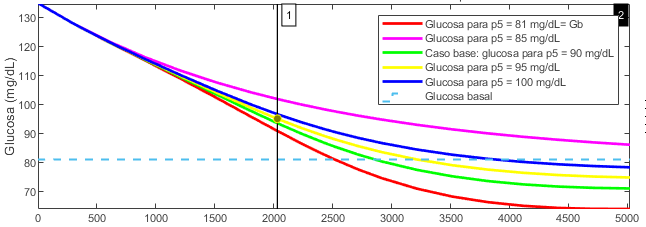
\includegraphics[width=\linewidth]{img/modelo_original/p5_var/amplio_p5_95.PNG}
        \caption{Glucosa para $p_5$.}
        \label{fig:p5_gluc_zoom}
    \end{subfigure}
    
    \vspace{0.5cm} % Espacio vertical entre las subfiguras

    \begin{subfigure}[b]{0.9\linewidth} % Ancho ajustado al 90% del ancho de la línea
        \centering
        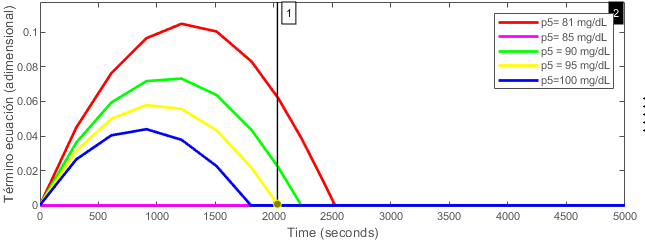
\includegraphics[width=\linewidth]{img/modelo_original/p5_var/amplio_p5_95-adi.PNG}
        \caption{Término adimensional para $p_5$.}
        \label{fig:p5_adi_zoom}
    \end{subfigure}
    
    \caption{Correlación entre la glucosa y el término adimensional de la insulina para el umbral $p_5$ en el Modelo de Bergman. Fuente propia.}
    \label{fig:zoom_p5}
\end{figure}


Se observa para la curva amarilla (correspondiente a $p_5$ =95 mg/dL) cómo en el instante en el que G(t) alcanza este valor, el término de la ecuación de la insulina se vuelve 0. Esto se debe a que la diferencia G(t) - $p_5$ se hace nula, y por tanto, su parte positiva también lo es.
Esta situación indica que, al alcanzar el valor umbral de 95 mg/dL, el estímulo para la liberación de insulina se detiene inmediatamente. En otras palabras, el páncreas deja de secretar insulina porque la concentración de glucosa ha bajado al nivel basal o por debajo de este. Este cese en la liberación de insulina no se refleja instantáneamente en la concentración de insulina I(t), ya que hay un pequeño retraso antes de que comience a disminuir, visible en la Figura \ref{fig:p5_ins}. El comportamiento aquí presente se reproduce para todos los casos simulados.

\clearpage
De la misma forma, se ha considerado realizar un pequeño análisis de los parámetros $p_1$, $p_2$ y $p_3$ del modelo. Los valores empleados se recogen en la tabla incluida en el anexo.

El efecto más significativo en la glucosa para la variación de estos parámetros se ha producido en la \textbf{tasa de eliminación de la glucosa, $p_1$}.

\begin{figure}[htbp]
    \centering
    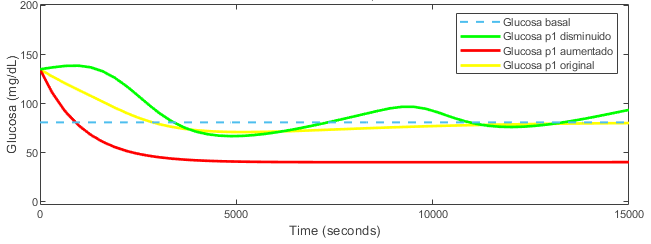
\includegraphics[width=0.9\linewidth]{img/modelo_original/p1_gl.png}
    \caption{Efecto en la glucosa de la variación de $p_1$. Fuente propia.}
    \label{fig:p1_gluc}
\end{figure}
\begin{figure}[htbp]
    \centering
    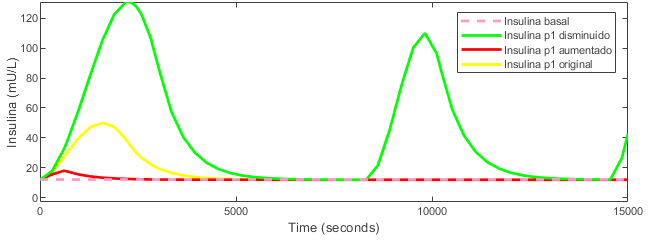
\includegraphics[width=0.9\linewidth]{img/modelo_original/p1_ins.png}
    \caption{Efecto en la glucosa de la variación de $p_1$. Fuente propia.}
    \label{fig:p1_ins}
\end{figure}

Valores \textit{aumentados de $p_1$} pueden conducir a hipoglucemia, pues al eliminarse una mayor cantidad de glucosa, sus niveles se estabilizarán por debajo de los basales, lo que representaría un importante riesgo para el paciente.  Valores \textit{disminuidos de $p_1$} conllevan a una menor velocidad de eliminación de glucosa, lo que puede resultar en oscilaciones prolongadas de los niveles de glucosa, perdiendo la capacidad para estabilizarse en un valor estacionario.
Este comportamiento se ratifica a nivel insulínico, donde valores aumentados de p1 muestran la poca necesidad de liberación de insulina por parte del páncreas, pues los niveles de glucosa son bajos. Por el contrario, valores muy disminuidos de p1 generan una respuesta anormal del organismo, no viable, donde los niveles de insulina se disparan de forma muy pronunciada. Además, no llegan a estabilizarse en un nivel basal próximo a Ib.

Los efectos de los parámetros $p_2$ y $p_3$, por ser menos significativos, se incluyen en el anexo.

\section{Comportamiento glucémico alterado}

Se muestra a continuacion el comportamiento del sistema glucorregulatorio de un \textbf{paciente diabético}. Se ha considerado llevar a cabo este análisis empleando un paciente diabético tipo 1. Su condición insulínica (de déficit absoluto), que se ha considerado “más extrema” que la presente en la diabetes tipo 2, se estima que puede reflejar mejor el comportamiento del organismo cuando la interacción glucosa – insulina se encuentra desajustada. Por tanto, se trabajará con un paciente que requiere de administración de insulina exógena (mediante el sistema de ecuaciones \ref{eq:ecBergMod} del Modelo de Bergman Modificado), pues es incapaz de producir insulina por si mismo, y, de no ser por esta administración, no podría mantener los rangos de glucosa en valores saludables. 

\subsection{Variación de la constante de tiempo n}

Como se ha indicado en la Sección \ref{sec:indicar_n}, la constante de tiempo n indica el tiempo que tarda la insulina en alcanzar el valor de la insulina exógena administrada (cte.). Pese a que para este estudio se considera el valor especificado en la Tabla \ref{tab:parametros_glucemicos}, se pretende observar si la modificación de este parámetro supone diferencias significativas en el comportamiento de la glucosa e insulina.  Se considera la insulina exógena U calculada en el apartado \ref{sec:insulina_calculo}.

Para esta simulación, se estima lo siguiente:
\begin{align}
    \text{- Si n es muy pequeño: } \frac{1}{n \downarrow} =  \uparrow \text{el tiempo para alcanzar la insulina administrada}\\
    \text{- Si n es muy grande: } \frac{1}{n \uparrow} =  \downarrow \text{el tiempo para alcanzar la insulina administrada}
\end{align}

\clearpage
\begin{figure}[htbp]
    \centering
    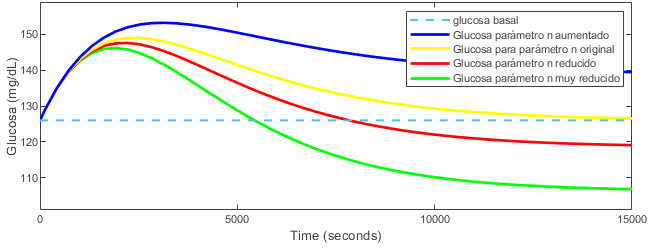
\includegraphics[width=0.9\linewidth]{img/modelo_modificado/variacion_n/n_gluco.png}
    \caption{Comportamiento de la glucosa para diferentes valores del parámetro n. Fuente propia.}
    \label{fig:n_gluc_bergm_mod}
\end{figure}
\begin{figure}[htbp]
    \centering
    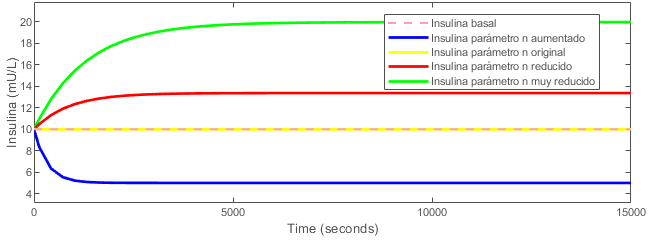
\includegraphics[width=0.9\linewidth]{img/modelo_modificado/variacion_n/n_ins.png}
    \caption{Comportamiento de la insulina para diferentes valores del parámetro n. Fuente propia.}
    \label{fig:n_ins_bergm_mod}
\end{figure}

Como se observa en las gráficas, para la insulina (Figura \ref{fig:n_ins_bergm_mod}), valores inferiores al original aumentan el tiempo que tarda la insulina en alcanzar el nivel adecuado de insulina administrada, lo que se traduce en la gráfica como una reducción de la pendiente que a su vez tarda más en estabilizarse, pues la insulina se elimina más lentamente. La mayor cantidad de insulina presente en el organismo hace que la glucosa se estabilice en un nivel más bajo que el basal. Para valores aumentados de n, la insulina se elimina más rápidamente, lo que conlleva a una disminución de la concentración de insulina en sangre. La menor cantidad de insulina disponible es menos efectiva en reducir los niveles de glucosa, lo que lleva a una estabilización en un nivel de glucosa más alto. El efecto de ello se observa en la Figura \ref{fig:n_gluc_bergm_mod} para la glucosa.


\subsection{Perturbaciones y entradas}

La ingesta se incluye en el Modelo de Bergman Modificado altamente unida al tiempo, pues delimitamos el efecto de la ingesta estableciendo un t determinado de duración de estos efectos. 
Para los ejemplos que se incluyen a continuación, se compara la ingesta de 50 y 75 gramos de carbohidratos. La gráfica de la Figura \ref{fig:ingesta_solo} muestra el comportamiento de la ingesta, y cómo, si aumentas la cantidad de carbohidratos ingeridos, la curva alcanza niveles superiores. Se observa además, que, la ingesta, una vez termina la duración del efecto, vuelve a 0, pues ya no hay resto de carbohidratos en el organismo.

\begin{figure}[htbp]
    \centering
    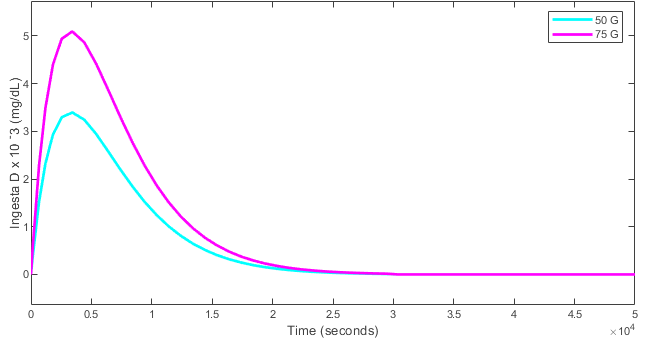
\includegraphics[width=0.9\linewidth]{img/modelo_modificado/casos base e ingesta/ingesta_sol.png}
    \caption{Curva de la función ingesta para el modelo. Fuente propia.}
    \label{fig:ingesta_solo}
\end{figure}

Para un paciente diabético, al que no le administramos insulina exógena, se obtiene un nivel en el que se estabiliza la glucosa superior a Gb (Figura \ref{fig:ingesta_glucosa}), mostrando un comportamiento incorrecto en términos regulatorios. Por tanto, si a este paciente le administramos la suficiente insulina exógena, sus niveles de glucosa volverán, tras la ingesta, a su basal Gb, así como se contribuirá a disminuir el pico máximo de glucosa.
\clearpage
\begin{figure}[htbp]
    \centering
    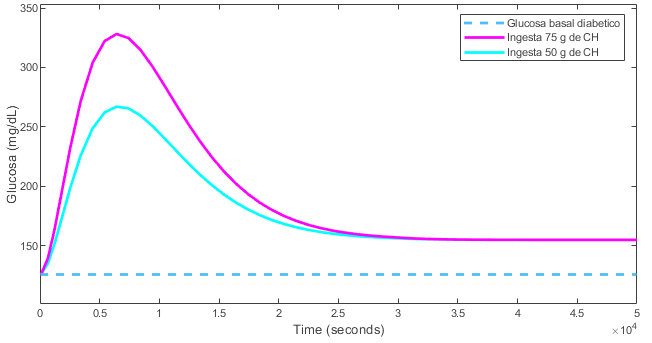
\includegraphics[width=0.9\linewidth]{img/modelo_modificado/casos base e ingesta/ing_gluc.png}
    \caption{Efecto de la ingesta en la glucosa para pacientes diabéticos. Fuente propia.}
    \label{fig:ingesta_glucosa}
\end{figure}

\underline{La insulina exógena} 

Se modela a continuación, por tanto, el comportamiento de la glucosa en sangre del paciente en ayunas considerando la insulina exógena U, como parámetro constante, reflejando, de forma relativa, el mecanismo de la insulina de acción prolongada en el organismo. 

En la Figura \ref{fig:dosis_ins} se simula el comportamiento de la glucosa y la insulina para el paciente en ayunas, bajo diferentes dosis de insulina exógena. Se observa una relación inversamente proporcional de la insulina exógena y el nivel de glucosa en sangre: cuanta más insulina externa recibe el paciente, menores serán sus niveles de glucosa en sangre. Excesos en la administración de esta insulina pueden provocar que los niveles de glucosa del paciente caigan por debajo de su nivel basal Gb, causando hipoglucemias. Por otro lado, si la insulina externa es insuficiente, los niveles de glucosa se ven aumentados llegando a causar hiperglucemias, sin alcanzar tampoco los niveles basales de glucosa. 
\clearpage
\begin{figure}[htbp]
    \centering
    \begin{subfigure}[b]{0.9\linewidth} % Ancho ajustado al 90% del ancho de la línea
        \centering
        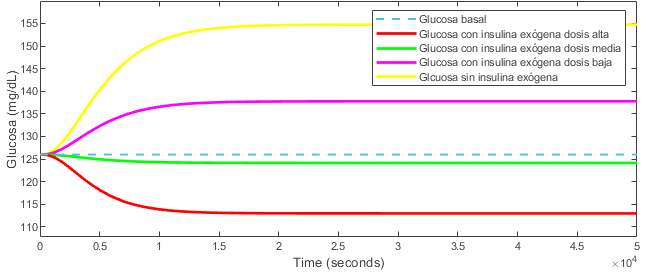
\includegraphics[width=\linewidth]{img/modelo_modificado/casos insulina/dosis_base.png}
        \caption{Glucosa con diferentes dosis de insulina exógena.}
    \end{subfigure}
    
    \vspace{0.5cm} % Espacio vertical entre las subfiguras

    \begin{subfigure}[b]{0.9\linewidth} % Ancho ajustado al 90% del ancho de la línea
        \centering
        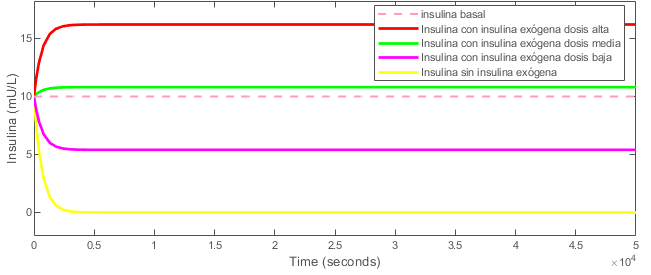
\includegraphics[width=\linewidth]{img/modelo_modificado/casos insulina/dosis_base_insul.png}
        \caption{Insulina con diferentes dosis de insulina exógena.}
    \end{subfigure}
    
    \caption{Comparativa del comportamiento de la glucosa e insulina para diferentes dosis de insulina exógena. Fuente propia.}
    \label{fig:dosis_ins}
\end{figure}


Así, administrando al paciente la dosis de insulina exógena exacta calculada para lograr que G(t)=Gb, se logra el correcto comportamiento del sistema glucorregulatorio tras la ingesta en la Figura \ref{fig:ins_ex_ing}.

Se comprueba que para este paciente, la cantidad de insulina administrada es suficiente para regular sus niveles de glucosa en sangre en ambas situaciones. Esta administración por tanto podría considerarse de insulina de acción prolongada (Sección \ref{sec:ins_prol}), donde sus efectos tienen una duración de 18-24 h, y son suficientes para estabilizar al paciente en su valor basal.
\clearpage
\begin{figure}[htbp]
    \centering
    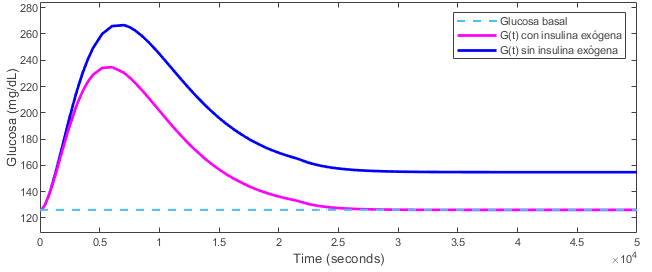
\includegraphics[width=0.9\linewidth]{img/modelo_modificado/casos insulina/ins_exacta_ing.png}
    \caption{Efecto en la glucosa de la administración adecuada de insulina externa para una ingesta. Fuente propia.}
    \label{fig:ins_ex_ing}
\end{figure}


\begin{itemize}
    \item Insulina rápida
\end{itemize}
Se ha tratado de simular el comportamiento de la insulina de acción rápida en el organismo, así como su efecto en los niveles glucémicos. Para ello se ha explorado un caso que implica la administración de insulina exógena de manera progresiva justo antes de la ingesta de alimentos. Para realizar este cálculo, se considera el tiempo necesario para que este tipo de insulina comience a actuar, el cual, como se ha indicado en la Sección \ref{sec:ins_rap}, oscila entre 5 y 20 minutos. En este contexto, se selecciona un tiempo de acción inicial de 10 minutos antes de la ingesta, alcanzando el pico de concentración de insulina administrada en 1 hora y media. Se estima que, a partir de este punto, la concentración se mantendrá constante hasta que comience a disminuir, eliminándose su efecto en un rango de 4 a 6 horas.
La ejecución de esta simulación no refleja la realidad de manera precisa, ya que este efecto “rampa” simula un comportamiento como si se administrara un porcentaje de la dosis por unidad de tiempo, aumentando progresivamente hasta alcanzar un máximo, para luego disminuir hasta llegar a cero. En la práctica clínica, el paciente se administra una inyección en un momento específico, pero para este modelo, dicho enfoque no produciría resultados significativos. A pesar de esto, el efecto de esta simulación se asemeja considerablemente al impacto que tiene la insulina rápida sobre los niveles de glucosa, justificando así la inclusión de este apartado en el estudio.
\clearpage
\begin{figure}[htbp]
    \centering
    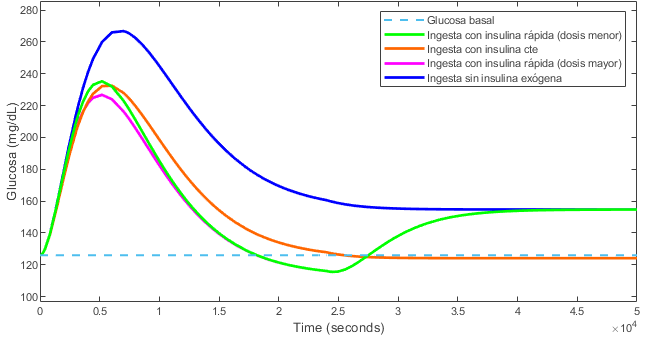
\includegraphics[width=0.9\linewidth]{img/modelo_modificado/casos insulina/caso_rapida.png}
    \caption{Efecto en la glucosa de la administración de insulina rápida y cte. Fuente propia.}
    \label{fig:ins_rap_const}
\end{figure}

Para la simulación de la insulina rápida de la Figura \ref{fig:ins_rap_const}, se observan diferencias en cuanto a la estabilización de los niveles de glucosa en el nivel basal. Para los casos de administración de insulina rápida, la glucosa logra reducir su curva considerablemente, alcanzando prácticamente los resultados de la administración de insulina cte. La pendiente de esta curva disminuye a valores inferiores a Gb, lo que indica que malas regulaciones de las dosis insulínicas puede desencadenar efectos como hipoglucemias, pese a que para este caso se encuentra dentro de límites adecuados. No se observan diferencias significativas entre las dosis de insulina rápida simuladas. Sin embargo, debido a la duración de la acción de la insulina, se observa cómo, una vez finaliza su efecto, los valores glucémicos comienzan a aumentar de nuevo, reflejando el comportamiento alterado del sistema. 

Por ello se estima simular otro caso en el que se combina la acción de la insulina rápida con la constante (Figura \ref{fig:comb_rap_cte}) con la finalidad de observar sus efectos en el sistema regulatorio.  Cabe destacar que el propósito de esta simulación es exclusivamente académico y no pretende establecer recomendaciones clínicas sobre qué tipo de insulina es mejor.
Los resultados muestran que la combinación de insulina constante con insulina rápida produce un menor pico glucémico comparado con la administración de insulina rápida por sí sola. Además, la insulina constante ayuda a estabilizar G(t) en su valor basal. Este comportamiento sugiere que la combinación de ambos tipos de insulina podría ser útil en escenarios donde la insulina prolongada por sí sola no logra reducir los picos máximos de glucosa de manera efectiva. Sin embargo, es importante resaltar que estos resultados no deben interpretarse como recomendaciones clínicas, sino como una exploración de los efectos de diferentes variables en el sistema regulatorio de la glucosa.

\begin{figure}[htbp]
    \centering
    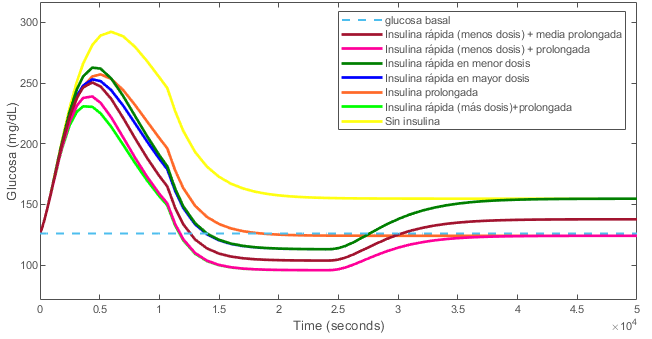
\includegraphics[width=0.9\linewidth]{img/modelo_modificado/casos insulina/combinacion.png}
    \caption{Efecto en la glucosa de la combinación en la administración de insulina rápida y cte. Fuente propia.}
    \label{fig:comb_rap_cte}
\end{figure}

\underline{El ejercicio físico} 

Se estudia el efecto en los niveles de glucosa de realizar ejercicio físico, así como la estimación del momento del día optimo para llevarlo a cabo. Se trabaja bajo la suposición de una ausencia de inyección de insulina exógena en el organismo con la finalidad de observar el efecto de la variable del ejercicio de forma aislada. La ingesta de las simulaciones contiene 50 g de carbohidratos y comienza a las 3 horas del inicio de la simulación. El ejercicio físico dura 1,2 o 3 horas, y el paciente tiene una glucosa inicial igual a su basal. Se muestran las gráficas correspondientes a la ingesta, al ejercicio y a la glucosa en sangre para el paciente.

Para los casos previos a la ingesta, estudiados en la Figura \ref{fig:ej_antes}, se observa que el efecto del ejercicio físico presenta una relación lineal, ya que a más ejercicio, menor valor de glucosa. Los casos tras ingesta de la Figura \ref{fig:ej_despues}, si que muestran relaciones diferentes entre ellos. Concretamente, cuanto antes comienza el ejercicio, más rápido disminuyen los niveles de glucosa en sangre. Además, al igual que en el caso anterior, la plena estabilización del sistema en el Gb solo ocurre para un periodo muy largo de ejercicio. 

\begin{figure}[htbp]
    \centering
    \begin{subfigure}[b]{0.9\linewidth} % Ancho ajustado al 90% del ancho de la línea
        \centering
        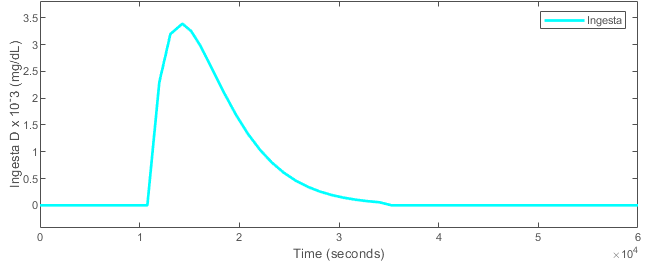
\includegraphics[width=\linewidth]{img/modelo_modificado/ejercicio/ingesta_prod.png}
        \caption{Curva de ingesta.}
    \end{subfigure}
    
    \vspace{0.5cm} % Espacio vertical entre las subfiguras

    \begin{subfigure}[b]{0.9\linewidth} % Ancho ajustado al 90% del ancho de la línea
        \centering
        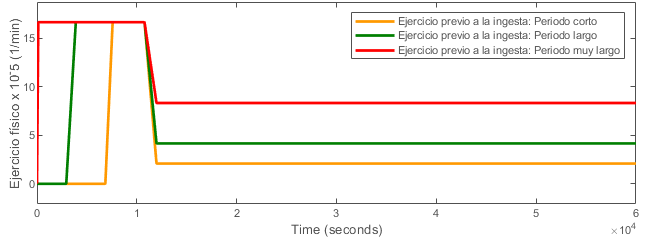
\includegraphics[width=\linewidth]{img/modelo_modificado/ejercicio/ejercicio_graf_previo.png}
        \caption{Ejercicio físico.}
    \end{subfigure}
    
    \vspace{0.5cm} % Espacio vertical entre las subfiguras

    \begin{subfigure}[b]{0.9\linewidth} % Ancho ajustado al 90% del ancho de la línea
        \centering
        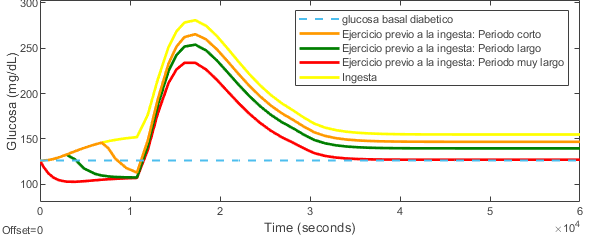
\includegraphics[width=\linewidth]{img/modelo_modificado/ejercicio/PREVIO.png}
        \caption{Curva de la glucosa.}
    \end{subfigure}
    
    \caption{Comparativa del comportamiento de la glucosa para diferentes tipos de ejercicio previos a la ingesta. Fuente propia.}
    \label{fig:ej_antes}
\end{figure}

\clearpage
\begin{figure}[htbp]
    \centering
    \begin{subfigure}[b]{0.9\linewidth} % Ancho ajustado al 90% del ancho de la línea
        \centering
        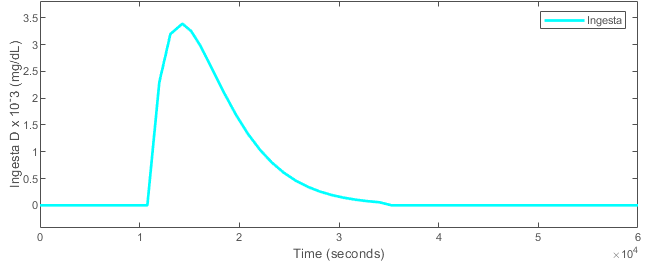
\includegraphics[width=\linewidth]{img/modelo_modificado/ejercicio/ingesta_prod.png}
        \caption{Curva de ingesta.}
    \end{subfigure}
    
    \vspace{0.5cm} % Espacio vertical entre las subfiguras

    \begin{subfigure}[b]{0.9\linewidth} % Ancho ajustado al 90% del ancho de la línea
        \centering
        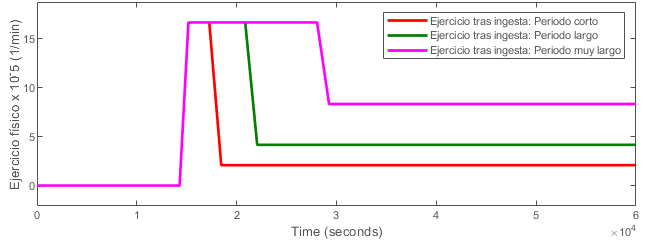
\includegraphics[width=\linewidth]{img/modelo_modificado/ejercicio/ejercicio_graf_tras.png}
        \caption{Ejercicio físico.}
    \end{subfigure}
    
    \vspace{0.5cm} % Espacio vertical entre las subfiguras

    \begin{subfigure}[b]{0.9\linewidth} % Ancho ajustado al 90% del ancho de la línea
        \centering
        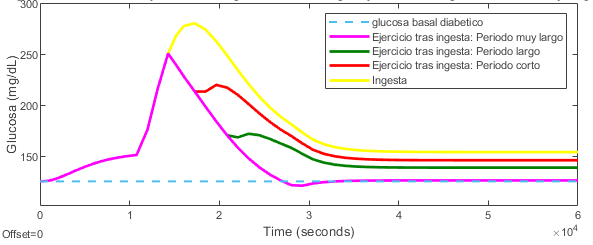
\includegraphics[width=\linewidth]{img/modelo_modificado/ejercicio/TRAS.png}
        \caption{Curva de la glucosa.}
    \end{subfigure}
    
    \caption{Comparativa del comportamiento de la glucosa para diferentes tipos de ejercicio tras la ingesta. Fuente propia.}
    \label{fig:ej_despues}
\end{figure}

\clearpage

\begin{itemize}
    \item Ejercicio físico e insulina
\end{itemize}

Pese a que, como se ha comprobado, la realización de ejercicio puede suponer mejoras en los niveles de glucosa, mediante los casos simulados no se logra retornar al valor basal a no ser que se aumente de forma considerable la duración del ejercicio. Se ha estimado por tanto estudiar una posible combinación entre ejercicio físico e insulina. 

Se incorpora la insulina exógena calculada anteriormente, que representa la \textit{dosis original} de insulina externa. Se estudian en este apartado diferentes proporciones de esta dosis, y se comparan con la realización de ejercicio físico. Para ello, se parte de periodos de ejercicio cortos y medios de las Figuras \ref{fig:ej_antes} y \ref{fig:ej_despues}, donde no se alcanzan los niveles basales de glucosa tras la ingesta. Es decir, la primera de las figuras compara la administración de diferentes cantidades de insulina exógena con la realización de \textbf{\textit{ejercicio corto}}, mientras que la segunda figura lleva a cabo esta comparación de dosis con el \textbf{\textit{ejercicio moderado}}.

Se observa que, para un periodo corto de ejercicio (Figura \ref{fig:ins+ej1}), no es necesaria una dosis completa de insulina. La curva morada estima que con 2/3 de la dosis original se alcanza el valor basal de glucosa, logrando estabilizarse. Para un periodo medio de ejercicio (Figura \ref{fig:ins+ej2}), la hipótesis era que se requeriría de una menor cantidad de la dosis inicial. Según las simulaciones, esta hipótesis es correcta, siendo necesaria únicamente media dosis de insulina para lograr que el paciente se estabilice en valores basales.

\begin{figure}[htbp]
    \centering
    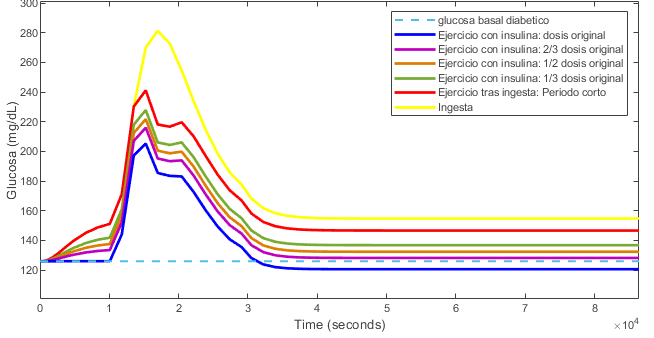
\includegraphics[width=0.9\linewidth]{img/modelo_modificado/ejercicio/ins+ej1.png}
    \caption{Efecto en la glucosa de la combinación de un periodo corto de ejercicio físico con distintas dosis insulínicas. Fuente propia.}
    \label{fig:ins+ej1}
\end{figure}
\clearpage
\begin{figure}[htbp]
    \centering
    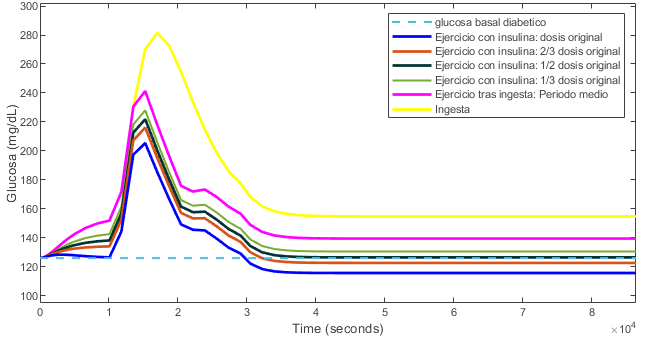
\includegraphics[width=0.9\linewidth]{img/modelo_modificado/ejercicio/ins+ej2.png}
    \caption{Efecto en la glucosa de la combinación de un periodo medio de ejercicio físico con distintas dosis insulínicas. Fuente propia.}
    \label{fig:ins+ej2}
\end{figure}

\section{Regulación del sistema glucosa - insulina}
\subsection{Métodos de sintonía}

Se muestran a continuación los resultados obtenidos para los dos métodos de sintonía empleados para el desarrollo del regulador: método de prueba y error, y método basado en experimentos.

\subsubsection{Método de Prueba y Error}

Para el Método de Prueba y Error, se han estimado valores para los términos proporcional e integral, concretamente, se ha desarrollado un regulador P y otro PI. En la Figura \ref{fig:prueba_error} se muestra la comparación entre ambos reguladores, así como con la administración de insulina exógena de forma manual, respecto a la ingesta sin insulina externa. 
\clearpage
\begin{figure}[htbp]
    \centering
    \begin{subfigure}[b]{0.9\linewidth} % Ancho ajustado al 90% del ancho de la línea
        \centering
        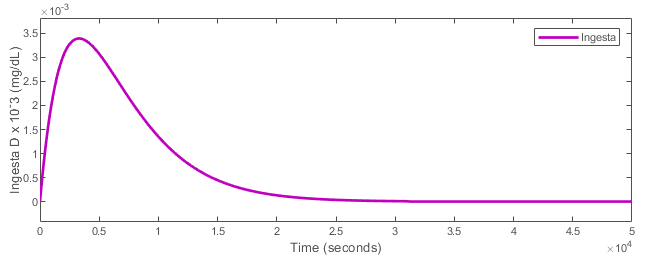
\includegraphics[width=\linewidth]{img/regulacion2/ingesta_p_e.png}
        \caption{Curva de la ingesta.}
    \end{subfigure}
    
    \vspace{0.5cm} % Espacio vertical entre las subfiguras

    \begin{subfigure}[b]{0.9\linewidth} % Ancho ajustado al 90% del ancho de la línea
        \centering
        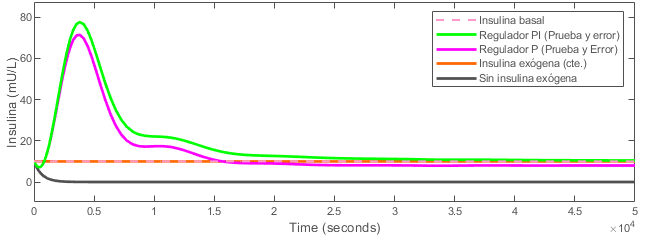
\includegraphics[width=\linewidth]{img/regulacion2/insulina_p_e.png}
        \caption{Curva de la insulina.}
    \end{subfigure}
    
    \vspace{0.5cm} % Espacio vertical entre las subfiguras

    \begin{subfigure}[b]{0.9\linewidth} % Ancho ajustado al 90% del ancho de la línea
        \centering
        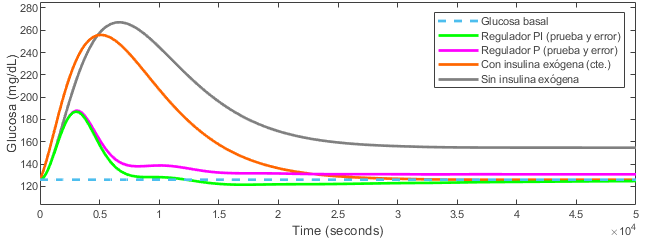
\includegraphics[width=\linewidth]{img/regulacion2/glucosa_p_e.png}
        \caption{Curva de la glucosa.}
    \end{subfigure}
    
    \caption{Gráfica de la ingesta y efecto en la insulina y la glucosa de los reguladores P y PI obtenidos mediante el Método de Prueba y Error. Fuente propia.}
    \label{fig:prueba_error}
\end{figure}

\clearpage
Como cabía esperar, tal y como se ha mencionado en la Sección \ref{sec:problematica_P} sobre la problemática del regulador proporcional, éste no es capaz de estabilizarse en valores basales, y requiere de la adición del término integral I para lograr un comportamiento adecuado. Se comprueba además que los reguladores obtenidos mediante este método de sintonía mejoran considerablemente la respuesta respecto a la administración de insulina considerada.

\begin{itemize}
    \item Variación del término P del regulador
\end{itemize}

Estudiando la variación del término proporcional en el regulador en la Figura \ref{fig:variacion_p}, cuyo ajuste óptimo es crucial para el correcto funcionamiento del sistema de regulación, se comprueba lo mencionado anteriormente. Aumentando este término respecto a su valor original, obtenemos oscilaciones en la respuesta de la glucosa, lo que puede ser perjudicial para el funcionamiento adecuado del organismo. La glucosa tiende a estabilizarse más rápidamente, pero a riesgo de presentar estas oscilaciones o sobreimpulsos debido a la respuesta más agresiva del regulador. El sistema puede volverse, así, menos estable. Por otro lado, para valores disminuidos de P, la glucosa se estabiliza más lentamente, pero la transición es más suave, con menos oscilaciones y un comportamiento más estable. Sin embargo, la gráfica de la glucosa adquiere una amplitud mucho más elevada, lo que se traduce en niveles de azúcar en sangre excesivamente altos, pudiendo causar hiperglucemias.

\begin{figure}[htbp]
    \centering
    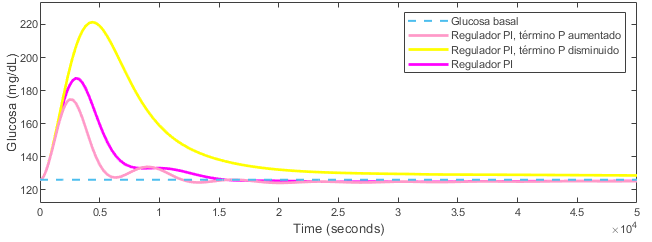
\includegraphics[width=0.9\linewidth]{img/regulacion/variacion_p.png}
    \caption{Efecto en la glucosa de la variación del término proporcional del regulador. Fuente propia.}
    \label{fig:variacion_p}
\end{figure}



\subsubsection{Método Basado en Experimentos}

Se recogen por último los dos reguladores sintonizados mediante el método basado en experimentos, que se diferencian en la inclusión en uno de ellos del término derivativo D. La teoría dice que añadir el término derivativo anticipa la respuesta, y permite ser mas eficiente rechazando la perturbación. De hecho, con un regulador PID se disminuye el valor del pico máximo y el tiempo en volver a la referencia. 

\begin{figure}[htbp]
    \centering
    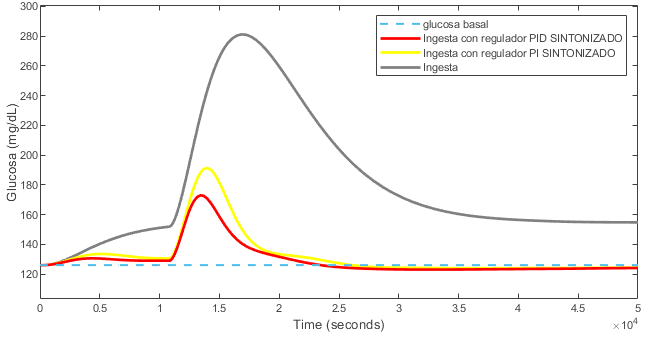
\includegraphics[width=0.9\linewidth]{img/regulacion/SINTONIZADO_PI_PID.png}
    \caption{Comparación de los reguladores sintonizados PI y PID y su efecto en la glucosa. Fuente propia.}
    \label{fig:sintonizado_PID}
\end{figure}

Se compara en la Figura \ref{fig:ejercicio_PID} el regulador PID obtenido mediante este método (en la Figura \ref{fig:sintonizado_PID}) con los casos de ejercicio físico estudiados anteriormente. Concretamente, se compara el mejor resultado de cada tipo de ejercicio (periodo muy largo, previo y tras la ingesta) con el regulador PID.

Como se puede observar, los niveles glucémicos obtenidos mediante el regulador PID son considerablemente mejores que para el resto de los casos. No solo el pico de la curva es considerablemente menor (reduciendo así el riesgo de hiperglucemias), sino que el sistema de control también permite reducir el tiempo de asentamiento de la curva, y logra estabilizarse antes en el nivel basal de glucosa.
\clearpage

\begin{figure}[htbp]
    \centering
    \begin{subfigure}[b]{0.9\linewidth} % Ancho ajustado al 90% del ancho de la línea
        \centering
        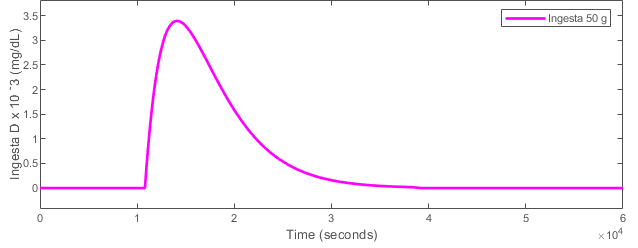
\includegraphics[width=\linewidth]{img/regulacion2/ingesta_comb.png}
        \caption{Curva de la ingesta.}
    \end{subfigure}
    
    \vspace{0.5cm} % Espacio vertical entre las subfiguras

    \begin{subfigure}[b]{0.9\linewidth} % Ancho ajustado al 90% del ancho de la línea
        \centering
        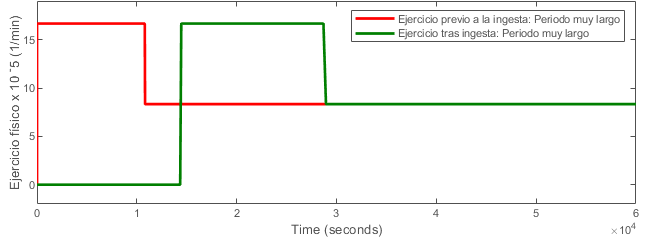
\includegraphics[width=\linewidth]{img/regulacion2/ejercicio_comb.png}
        \caption{Ejercicio físico.}
    \end{subfigure}
    
    \vspace{0.5cm} % Espacio vertical entre las subfiguras

    \begin{subfigure}[b]{0.9\linewidth} % Ancho ajustado al 90% del ancho de la línea
        \centering
        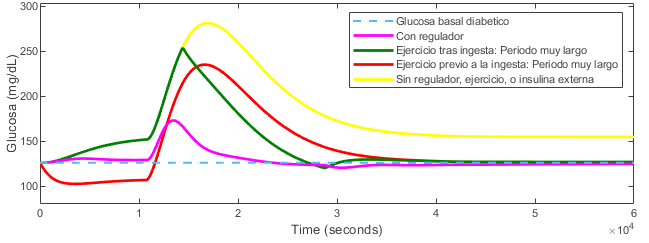
\includegraphics[width=\linewidth]{img/regulacion2/glucosa_comb.png}
        \caption{Curva de la glucosa.}
    \end{subfigure}
    
    \caption{Comparación del efecto en la glucosa del regulador PID y los mejores resultados de ejercicio físico. Fuente propia.}
    \label{fig:ejercicio_PID}
\end{figure}


Se muestra además en la Figura \ref{fig:graf_control_pid} la acción de control del regulador PID sintonizado, que se correspondería con la insulina exógena. Se comprueba cómo el regulador ejerce su efecto de control asemejándose al comportamiento de la administración de dicha insulina exógena de manera manual.
\clearpage
\begin{figure}[htbp]
    \centering
    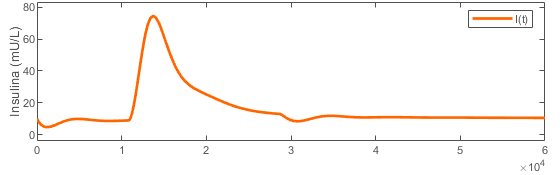
\includegraphics[width=0.9\linewidth]{img/regulacion/control_final.png}
    \caption{Evolución de la insulina y respuesta del controlador en un sistema de infusión de insulina. Fuente propia.}
    \label{fig:graf_control_pid}
\end{figure}

En el conjunto de reguladores obtenidos se comprueba el comportamiento de la glucosa frente a estos sistemas de control, que partiendo de valores iniciales que los definen, pueden ir modelando la glucosa para adecuarla dentro de los rangos no diabéticos.
A excepción de regulador P obtenido mediante el 'Método de Prueba y Error' en la Figura \ref{fig:prueba_error}, que, como se esperaba, no logra estibilizarse en valores basales de glucosa, el resto de reguladores han logrado respuestas adecuadas. Se comprueba cómo el pico glucémico se reduce significativamente (pasando de más de 240 a valores entorno a los 180 mg/dL) para todos los casos. Los mejores resultados se obtienen con el regulador PID sintonizado, como se esperaba, pues la adición del término derivativo permite al regulador anticiparse a los cambios en el error o la señal de control, mejorando así la respuesta dinámica del sistema. 

\subsection{Comparativa paciente sano y diabético}

Por último, se incluye en la Figura \ref{fig:comparacion_diab_no_diab} la comparativa del comportamiento de la glucosa entre un paciente no diabético y un paciente diabético (cuyos valores se encuentran en la Tabla \ref{tab:valores_finales_paciente}) al que se le modela la insulina exógena con la acción de un regulador.
El regulador empleado es el PID obtenido en la sección anterior.

Para esta simulación, se trata con dos hipotéticos pacientes que cuentan con los siguientes niveles basales de glucosa e insulina:

\begin{table}[htbp]
    \centering
    \caption{Valores basales estimados para los pacientes finales.}
    \begin{tabular}{|c|c|c|}
        \hline
          & Valor\\
        \hline
        Gb & 108 mg/dL \\
        Ib & 10 mU/L  \\
        \hline
    \end{tabular}
    \label{tab:valores_finales_paciente}
\end{table}

Además, comienzan con un nivel de glucosa de 171 mg/dL (tras una ingesta).

\begin{figure}[htbp]
    \centering
    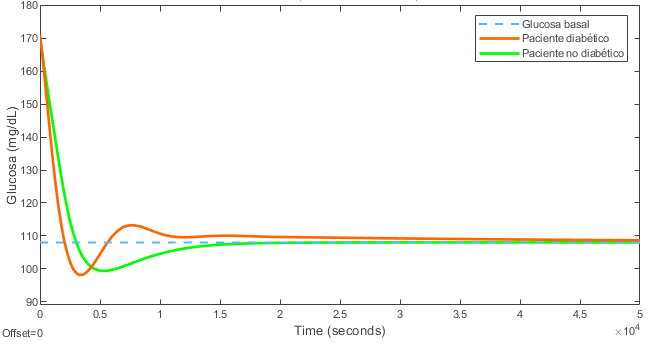
\includegraphics[width=0.9\linewidth]{img/regulacion/comparacion_no_diab.png}
    \caption{Comparación de los niveles de glucosa tras una ingesta de un paciente no diabético y un paciente diabético con regulador. Fuente propia.}
    \label{fig:comparacion_diab_no_diab}
\end{figure}

El regulador empleado sobre el paciente diabético hace que sus niveles de glucosa puedan estabilizarse en su nivel basal, de la misma forma que lo hace la administración manual de insulina exógena (incluso con mejores resultados). Para este paciente diabético, el regulador hace que la glucosa retorne a su valor basal en un tiempo de asentamiento algo menor si cabe que el propio funcionamiento del organismo del paciente no diabético. Se comprueba, por tanto, que un sistema de control en un paciente diabético permite conseguir una respuesta similar a la de un paciente sano, poniendo de manifiesto cómo es posible sustituir el comportamiento del páncreas por uno artificial.

\section{Discusión}

El modelado del sistema glucorregulatorio en el organismo llevado a cabo en este estudio ha tenido como finalidad observar el comportamiento de ciertas variables, como la glucosa e insulina, y el efecto en ellas al causar entradas y perturbaciones en el modelo, así como de los mecanismos de control.

Para un \textit{\textbf{paciente sano}}, no diabético, el comportamiento del modelo ha sido el esperado. Suponiendo inicialmente una insulina constante en el organismo, se ha mostrado cómo la glucosa mantiene constantes sus niveles en el caso de no producirse ninguna ingesta, así como los regula hasta estabilizarse en su nivel basal cuando se produce una ingesta. El modelo ha respondido bien ha esta perturbación. Sin embargo, esta hipótesis de insulina constante no se ajusta a la realidad, pues, pese a que esta variable ronda valores estables en ausencia de perturbación, el comportamiento propio del sistema no es estático, sino que es dinámico. Así, al realizar las simulaciones con la insulina variable respecto al tiempo, se observa el efecto de esta variación en las variables I(t) y X(t). Se comprueba cómo, cuando los niveles de glucosa en el organismo son elevados, se libera insulina, lo que causa un pico en la gráfica de la insulina I(t). Este cambio repercute directamente en la insulina activa, que se ve aumentada debido a la liberación de glucosa. 

Para este modelo de insulina variable se ha estudiado además el efecto de la variación del umbral del páncreas para la liberación de insulina. 
Se ha observado que valores disminuidos de $p_5$ causan una liberación más temprana de insulina ante aumentos de la glucosa, promoviendo una respuesta más rápida pero menos pronunciada en la reducción de los niveles de glucosa post-prandiales. Esta liberación de insulina lleva a la caída más temprana de sus niveles tras la ingesta, lo que podría afectar a la capacidad del organismo para mantener la glucosa en niveles normales durante peridos prolongados. Valores altos de $p_5$ se han traducido en una menor liberación de insulina, y se ha logrado una correcta estabilización de la glucosa e insulina para el paciente. Sin embargo, en casos diferentes al simulado, un aumento excesivo de este umbral puede ser perjudicial, pues el páncreas no liberará insulina hasta que los niveles de glucosa en sangre superen significativamente el umbral. Como resultado, la respuesta insulinémica se retrasará y podría ser insuficiente para manejar los aumentos moderados de glucosa después de las comidas, llegando a causar hiperglucemias.
Estos resultados subrayan la importancia crítica de calibrar correctamente el parámetro en modelos y tratamientos clínicos para garantizar una respuesta insulinémica óptima y una regulación efectiva de la glucosa.

Continuando con la importancia del ajuste de los parámetros del modelo, y teniendo en cuenta que en este estudio se ha empleado como valores originales de $p_1$, $p_2$ y $p_3$ los establecidos por Ficher en \cite{fisher1991semiclosed}, existe bastante heterogeneidad en su uso. El análisis de la variación de $p_1$, por ser el parámetro más significativo, ha estimado que un aumento en esta tasa de eliminación de glucosa puede llevar a una desestabilización del sistema por falta de glucosa en el organismo. Valores reducidos de este parámetro también causan este efecto, pero esta vez en forma de oscilaciones para la glucosa. Para la insulina, esta condición hace que se alcancen valores extremos de insulina en sangre, que son inaceptables para pacientes.

Respecto al comportamiento de la glucosa e insulina para \textit{\textbf{pacientes diabéticos}}, se ha mostrado cómo puede afectar de manera muy negativa la falta de tratamiento de la patología, resultando valores muy altos de glucosa que nunca llegan a estabilizarse. Este comportamiento se reproduce también para los casos de ingesta, pero muestra la relación contraria al incluir el ejercicio físico. Antes de hablar de esta perturbación, he considerado la administración de insulina exógena y el efecto que tiene en el organismo. Como es observable, la dosis insulínica para un paciente es única y atiende, entre otras cuestiones, a sus valores insulínicos, así como a su actividad. El ajuste adecuado de esta dosis es crucial para el tratamiento del paciente, pues de nada sirve esta administración si las dosis son excesivas, o altamente insuficientes. Cabe destacar que para este apartado la información encontrada en otras fuentes no ha sido la aquí presente, pues la insulina se incluye en la mayoría de los casos como valor constante, por lo que trato este punto como prueba experimental. En ocasiones, para los pacientes es suficiente con la insulina de acción prolongada, que mantiene su efecto durante todo el día y basta para estabilizar los niveles de glucosa en sangre. Otras veces, no es suficiente con ello, o bien se indica la administración de otro tipo de insulinas, por el efecto causado en el organismo, componentes y otras necesidades del paciente. Por ello se ha simulado también cómo sería el comportamiento de la insulina de acción rápida en el organismo, cuya implementación no está verificada pero que muestra un efecto en la glucosa acorde con el esperado. Se remarca además que no es la finalidad de este estudio proporcionar nuevas directrices o conclusiones sobre la dosificación óptima de la insulina en el organismo, sino estudiar las relaciones entre las variables y obtener comportamientos consecuentes con el sistema regulatorio. Una vez realizada esta consideración, en los resultados se puede observar que la insulina de acción rápida genera un efecto adecuado en la glucosa hasta que finaliza su dosis, donde la glucosa vuelve a sus valores atípicos. De ahí la importancia de estudiar cada caso por separado, pues, para el paciente simulado, no sería suficiente con esta insulina, ya que sus niveles de glucosa vuelven a aumentar por encima de Gb. La combinación de insulina rápida y prolongada (cte.) también se ha estudiado, de manera informativa, para comparar el efecto en los picos glucémicos de estos dos tipos de acciones. La combinación de ambas, como era esperado, es la que mejores resultados ha dado, logrando el pico menos pronunciado.
Respecto al ejercicio físico, se ha ratificado que provoca mejoras significativas en los niveles de glucosa en sangre. Aún así, es necesario recordar que esta variable se ha simulado con ecuaciones sencillas, que no representan completamente el comportamiento del organismo, sino que aportan una aproximación. Además, como se ha indicado previamente, la diabetes tipo 1 y el ejercicio pueden presentar riesgos, como la hipoglucemia. Una vez comentado este hecho, se ha estudiado el efecto generalizado del ejercicio antes y después de las comidas. Se ha seguido la hipótesis de que el ejercicio tras la ingesta era mejor que el previo a ella, y, en contra de lo esperado por mí, se ha cumplido esta hipótesis. Además, se ha cumplido la relación proporcional entre cantidad de ejercicio con mayor disminución de la glucosa. La interacción ejercicio e insulina se ha considerado para realizar una situación hipotética de combinación entre ambas variables con la finalidad de observar una reducción de los niveles de glucosa. De forma abstracta, se han considerado los casos de ejercicio moderado, que por si solos no logran retornar a los valores basales. Así, se ha determinado que para un periodo corto de tiempo de ejercicio, esta dosis sí podría verse reducida hasta en un tercio, mientras que realizando ejercicio durante un periodo medio se ha estimado una reducción de dosis mayor. Con estas demostraciones se ha pretendido verificar que las perturbaciones afectan de manera directa al sistema glucorregulatorio, de forma positiva o negativa.

Por último, en referencia a los \textit{\textbf{sistemas de control}} y mediante los métodos empleados, se comprueba que los sistemas de regulación insulínica suponen mejoras significativas, así como grandes avances en la tecnología médica. El diseño de los reguladores es un campo complejo y altamente específico en el que leves modificaciones pueden causar grandes desestabilizaciones en el sistema. Para los regulares simulados, se ha observado cómo la adición y combinación de los términos que componen el PID (Proporcional + Integral + Derivativo) causan efectos distintos. El regulador P, el más simple, aproxima su comportamiento al propio de la insulina externa en un acto de autorregulación. Un aumento de este término P disminuye el tiempo de asentamiento, es decir, disminuye el tiempo en el que la glucosa vuelve a su valor basal. Siendo este comportamiento positivo, y, pese a ello, P no logra estabilizarse en el punto basal porque el error de la acción de control nunca llega a ser cero. El regulador PI incluye un término integral que permite lograr la estabilización de G(t) y gestiona de forma adecuada el error, donde la acción de control u(t) sigue creciendo, aunque e(t) sea constante. Por otro lado, mediante métodos basados en experimentos ha sido posible sintonizar reguladores hallando el valor de sus términos mediante el método de López, mostrando otra forma de llevar a cabo este diseño. 

El comportamiento de los reguladores obtenidos presenta efectos positivos en la glucosa, a excepción del regulador P del "Método de Prueba y Error", que como se viene comentando, no llega a estabilizarse en Gb, por lo que en este caso, sería una opción descartada para el paciente. Los otros tres reguladores, destacando el regulador PID sintonizado, demuestran la capacidad del sistema de control para regular adecuadamente la curva de la glucosa, ajustando la insulina según las necesidades de la ingesta. La implementación de estos sistemas reduce considerablemente el tiempo de asentamiento de la curva, lo que supone una ventaja a la hora de evitar riesgos para el paciente. Comparando estos resultados con el comportamiento tras la ingesta de un paciente no diabético, se han logrado resultados muy similares. Este hecho sugiere que el uso de reguladores en la glucosa es altamente efectivo.